\documentclass[dvipsnames]{article} % For LaTeX2e  %dvipsnames for xcolor. otherwise this generates an error
\usepackage{iclr2023_conference,times}
\usepackage{xcolor}

% Optional math commands from https://github.com/goodfeli/dlbook_notation.
%%%%% NEW MATH DEFINITIONS %%%%%

\usepackage{amsmath,amsfonts,bm}

% Mark sections of captions for referring to divisions of figures
\newcommand{\figleft}{{\em (Left)}}
\newcommand{\figcenter}{{\em (Center)}}
\newcommand{\figright}{{\em (Right)}}
\newcommand{\figtop}{{\em (Top)}}
\newcommand{\figbottom}{{\em (Bottom)}}
\newcommand{\captiona}{{\em (a)}}
\newcommand{\captionb}{{\em (b)}}
\newcommand{\captionc}{{\em (c)}}
\newcommand{\captiond}{{\em (d)}}

% Highlight a newly defined term
\newcommand{\newterm}[1]{{\bf #1}}


% Figure reference, lower-case.
\def\figref#1{figure~\ref{#1}}
% Figure reference, capital. For start of sentence
\def\Figref#1{Figure~\ref{#1}}
\def\twofigref#1#2{figures \ref{#1} and \ref{#2}}
\def\quadfigref#1#2#3#4{figures \ref{#1}, \ref{#2}, \ref{#3} and \ref{#4}}
% Section reference, lower-case.
\def\secref#1{section~\ref{#1}}
% Section reference, capital.
\def\Secref#1{Section~\ref{#1}}
% Reference to two sections.
\def\twosecrefs#1#2{sections \ref{#1} and \ref{#2}}
% Reference to three sections.
\def\secrefs#1#2#3{sections \ref{#1}, \ref{#2} and \ref{#3}}
% Reference to an equation, lower-case.
\def\eqref#1{equation~\ref{#1}}
% Reference to an equation, upper case
\def\Eqref#1{Equation~\ref{#1}}
% A raw reference to an equation---avoid using if possible
\def\plaineqref#1{\ref{#1}}
% Reference to a chapter, lower-case.
\def\chapref#1{chapter~\ref{#1}}
% Reference to an equation, upper case.
\def\Chapref#1{Chapter~\ref{#1}}
% Reference to a range of chapters
\def\rangechapref#1#2{chapters\ref{#1}--\ref{#2}}
% Reference to an algorithm, lower-case.
\def\algref#1{algorithm~\ref{#1}}
% Reference to an algorithm, upper case.
\def\Algref#1{Algorithm~\ref{#1}}
\def\twoalgref#1#2{algorithms \ref{#1} and \ref{#2}}
\def\Twoalgref#1#2{Algorithms \ref{#1} and \ref{#2}}
% Reference to a part, lower case
\def\partref#1{part~\ref{#1}}
% Reference to a part, upper case
\def\Partref#1{Part~\ref{#1}}
\def\twopartref#1#2{parts \ref{#1} and \ref{#2}}

\def\ceil#1{\lceil #1 \rceil}
\def\floor#1{\lfloor #1 \rfloor}
\def\1{\bm{1}}
\newcommand{\train}{\mathcal{D}}
\newcommand{\valid}{\mathcal{D_{\mathrm{valid}}}}
\newcommand{\test}{\mathcal{D_{\mathrm{test}}}}

\def\eps{{\epsilon}}


% Random variables
\def\reta{{\textnormal{$\eta$}}}
\def\ra{{\textnormal{a}}}
\def\rb{{\textnormal{b}}}
\def\rc{{\textnormal{c}}}
\def\rd{{\textnormal{d}}}
\def\re{{\textnormal{e}}}
\def\rf{{\textnormal{f}}}
\def\rg{{\textnormal{g}}}
\def\rh{{\textnormal{h}}}
\def\ri{{\textnormal{i}}}
\def\rj{{\textnormal{j}}}
\def\rk{{\textnormal{k}}}
\def\rl{{\textnormal{l}}}
% rm is already a command, just don't name any random variables m
\def\rn{{\textnormal{n}}}
\def\ro{{\textnormal{o}}}
\def\rp{{\textnormal{p}}}
\def\rq{{\textnormal{q}}}
\def\rr{{\textnormal{r}}}
\def\rs{{\textnormal{s}}}
\def\rt{{\textnormal{t}}}
\def\ru{{\textnormal{u}}}
\def\rv{{\textnormal{v}}}
\def\rw{{\textnormal{w}}}
\def\rx{{\textnormal{x}}}
\def\ry{{\textnormal{y}}}
\def\rz{{\textnormal{z}}}

% Random vectors
\def\rvepsilon{{\mathbf{\epsilon}}}
\def\rvtheta{{\mathbf{\theta}}}
\def\rva{{\mathbf{a}}}
\def\rvb{{\mathbf{b}}}
\def\rvc{{\mathbf{c}}}
\def\rvd{{\mathbf{d}}}
\def\rve{{\mathbf{e}}}
\def\rvf{{\mathbf{f}}}
\def\rvg{{\mathbf{g}}}
\def\rvh{{\mathbf{h}}}
\def\rvu{{\mathbf{i}}}
\def\rvj{{\mathbf{j}}}
\def\rvk{{\mathbf{k}}}
\def\rvl{{\mathbf{l}}}
\def\rvm{{\mathbf{m}}}
\def\rvn{{\mathbf{n}}}
\def\rvo{{\mathbf{o}}}
\def\rvp{{\mathbf{p}}}
\def\rvq{{\mathbf{q}}}
\def\rvr{{\mathbf{r}}}
\def\rvs{{\mathbf{s}}}
\def\rvt{{\mathbf{t}}}
\def\rvu{{\mathbf{u}}}
\def\rvv{{\mathbf{v}}}
\def\rvw{{\mathbf{w}}}
\def\rvx{{\mathbf{x}}}
\def\rvy{{\mathbf{y}}}
\def\rvz{{\mathbf{z}}}

% Elements of random vectors
\def\erva{{\textnormal{a}}}
\def\ervb{{\textnormal{b}}}
\def\ervc{{\textnormal{c}}}
\def\ervd{{\textnormal{d}}}
\def\erve{{\textnormal{e}}}
\def\ervf{{\textnormal{f}}}
\def\ervg{{\textnormal{g}}}
\def\ervh{{\textnormal{h}}}
\def\ervi{{\textnormal{i}}}
\def\ervj{{\textnormal{j}}}
\def\ervk{{\textnormal{k}}}
\def\ervl{{\textnormal{l}}}
\def\ervm{{\textnormal{m}}}
\def\ervn{{\textnormal{n}}}
\def\ervo{{\textnormal{o}}}
\def\ervp{{\textnormal{p}}}
\def\ervq{{\textnormal{q}}}
\def\ervr{{\textnormal{r}}}
\def\ervs{{\textnormal{s}}}
\def\ervt{{\textnormal{t}}}
\def\ervu{{\textnormal{u}}}
\def\ervv{{\textnormal{v}}}
\def\ervw{{\textnormal{w}}}
\def\ervx{{\textnormal{x}}}
\def\ervy{{\textnormal{y}}}
\def\ervz{{\textnormal{z}}}

% Random matrices
\def\rmA{{\mathbf{A}}}
\def\rmB{{\mathbf{B}}}
\def\rmC{{\mathbf{C}}}
\def\rmD{{\mathbf{D}}}
\def\rmE{{\mathbf{E}}}
\def\rmF{{\mathbf{F}}}
\def\rmG{{\mathbf{G}}}
\def\rmH{{\mathbf{H}}}
\def\rmI{{\mathbf{I}}}
\def\rmJ{{\mathbf{J}}}
\def\rmK{{\mathbf{K}}}
\def\rmL{{\mathbf{L}}}
\def\rmM{{\mathbf{M}}}
\def\rmN{{\mathbf{N}}}
\def\rmO{{\mathbf{O}}}
\def\rmP{{\mathbf{P}}}
\def\rmQ{{\mathbf{Q}}}
\def\rmR{{\mathbf{R}}}
\def\rmS{{\mathbf{S}}}
\def\rmT{{\mathbf{T}}}
\def\rmU{{\mathbf{U}}}
\def\rmV{{\mathbf{V}}}
\def\rmW{{\mathbf{W}}}
\def\rmX{{\mathbf{X}}}
\def\rmY{{\mathbf{Y}}}
\def\rmZ{{\mathbf{Z}}}

% Elements of random matrices
\def\ermA{{\textnormal{A}}}
\def\ermB{{\textnormal{B}}}
\def\ermC{{\textnormal{C}}}
\def\ermD{{\textnormal{D}}}
\def\ermE{{\textnormal{E}}}
\def\ermF{{\textnormal{F}}}
\def\ermG{{\textnormal{G}}}
\def\ermH{{\textnormal{H}}}
\def\ermI{{\textnormal{I}}}
\def\ermJ{{\textnormal{J}}}
\def\ermK{{\textnormal{K}}}
\def\ermL{{\textnormal{L}}}
\def\ermM{{\textnormal{M}}}
\def\ermN{{\textnormal{N}}}
\def\ermO{{\textnormal{O}}}
\def\ermP{{\textnormal{P}}}
\def\ermQ{{\textnormal{Q}}}
\def\ermR{{\textnormal{R}}}
\def\ermS{{\textnormal{S}}}
\def\ermT{{\textnormal{T}}}
\def\ermU{{\textnormal{U}}}
\def\ermV{{\textnormal{V}}}
\def\ermW{{\textnormal{W}}}
\def\ermX{{\textnormal{X}}}
\def\ermY{{\textnormal{Y}}}
\def\ermZ{{\textnormal{Z}}}

% Vectors
\def\vzero{{\bm{0}}}
\def\vone{{\bm{1}}}
\def\vmu{{\bm{\mu}}}
\def\vtheta{{\bm{\theta}}}
\def\va{{\bm{a}}}
\def\vb{{\bm{b}}}
\def\vc{{\bm{c}}}
\def\vd{{\bm{d}}}
\def\ve{{\bm{e}}}
\def\vf{{\bm{f}}}
\def\vg{{\bm{g}}}
\def\vh{{\bm{h}}}
\def\vi{{\bm{i}}}
\def\vj{{\bm{j}}}
\def\vk{{\bm{k}}}
\def\vl{{\bm{l}}}
\def\vm{{\bm{m}}}
\def\vn{{\bm{n}}}
\def\vo{{\bm{o}}}
\def\vp{{\bm{p}}}
\def\vq{{\bm{q}}}
\def\vr{{\bm{r}}}
\def\vs{{\bm{s}}}
\def\vt{{\bm{t}}}
\def\vu{{\bm{u}}}
\def\vv{{\bm{v}}}
\def\vw{{\bm{w}}}
\def\vx{{\bm{x}}}
\def\vy{{\bm{y}}}
\def\vz{{\bm{z}}}

% Elements of vectors
\def\evalpha{{\alpha}}
\def\evbeta{{\beta}}
\def\evepsilon{{\epsilon}}
\def\evlambda{{\lambda}}
\def\evomega{{\omega}}
\def\evmu{{\mu}}
\def\evpsi{{\psi}}
\def\evsigma{{\sigma}}
\def\evtheta{{\theta}}
\def\eva{{a}}
\def\evb{{b}}
\def\evc{{c}}
\def\evd{{d}}
\def\eve{{e}}
\def\evf{{f}}
\def\evg{{g}}
\def\evh{{h}}
\def\evi{{i}}
\def\evj{{j}}
\def\evk{{k}}
\def\evl{{l}}
\def\evm{{m}}
\def\evn{{n}}
\def\evo{{o}}
\def\evp{{p}}
\def\evq{{q}}
\def\evr{{r}}
\def\evs{{s}}
\def\evt{{t}}
\def\evu{{u}}
\def\evv{{v}}
\def\evw{{w}}
\def\evx{{x}}
\def\evy{{y}}
\def\evz{{z}}

% Matrix
\def\mA{{\bm{A}}}
\def\mB{{\bm{B}}}
\def\mC{{\bm{C}}}
\def\mD{{\bm{D}}}
\def\mE{{\bm{E}}}
\def\mF{{\bm{F}}}
\def\mG{{\bm{G}}}
\def\mH{{\bm{H}}}
\def\mI{{\bm{I}}}
\def\mJ{{\bm{J}}}
\def\mK{{\bm{K}}}
\def\mL{{\bm{L}}}
\def\mM{{\bm{M}}}
\def\mN{{\bm{N}}}
\def\mO{{\bm{O}}}
\def\mP{{\bm{P}}}
\def\mQ{{\bm{Q}}}
\def\mR{{\bm{R}}}
\def\mS{{\bm{S}}}
\def\mT{{\bm{T}}}
\def\mU{{\bm{U}}}
\def\mV{{\bm{V}}}
\def\mW{{\bm{W}}}
\def\mX{{\bm{X}}}
\def\mY{{\bm{Y}}}
\def\mZ{{\bm{Z}}}
\def\mBeta{{\bm{\beta}}}
\def\mPhi{{\bm{\Phi}}}
\def\mLambda{{\bm{\Lambda}}}
\def\mSigma{{\bm{\Sigma}}}

% Tensor
\DeclareMathAlphabet{\mathsfit}{\encodingdefault}{\sfdefault}{m}{sl}
\SetMathAlphabet{\mathsfit}{bold}{\encodingdefault}{\sfdefault}{bx}{n}
\newcommand{\tens}[1]{\bm{\mathsfit{#1}}}
\def\tA{{\tens{A}}}
\def\tB{{\tens{B}}}
\def\tC{{\tens{C}}}
\def\tD{{\tens{D}}}
\def\tE{{\tens{E}}}
\def\tF{{\tens{F}}}
\def\tG{{\tens{G}}}
\def\tH{{\tens{H}}}
\def\tI{{\tens{I}}}
\def\tJ{{\tens{J}}}
\def\tK{{\tens{K}}}
\def\tL{{\tens{L}}}
\def\tM{{\tens{M}}}
\def\tN{{\tens{N}}}
\def\tO{{\tens{O}}}
\def\tP{{\tens{P}}}
\def\tQ{{\tens{Q}}}
\def\tR{{\tens{R}}}
\def\tS{{\tens{S}}}
\def\tT{{\tens{T}}}
\def\tU{{\tens{U}}}
\def\tV{{\tens{V}}}
\def\tW{{\tens{W}}}
\def\tX{{\tens{X}}}
\def\tY{{\tens{Y}}}
\def\tZ{{\tens{Z}}}


% Graph
\def\gA{{\mathcal{A}}}
\def\gB{{\mathcal{B}}}
\def\gC{{\mathcal{C}}}
\def\gD{{\mathcal{D}}}
\def\gE{{\mathcal{E}}}
\def\gF{{\mathcal{F}}}
\def\gG{{\mathcal{G}}}
\def\gH{{\mathcal{H}}}
\def\gI{{\mathcal{I}}}
\def\gJ{{\mathcal{J}}}
\def\gK{{\mathcal{K}}}
\def\gL{{\mathcal{L}}}
\def\gM{{\mathcal{M}}}
\def\gN{{\mathcal{N}}}
\def\gO{{\mathcal{O}}}
\def\gP{{\mathcal{P}}}
\def\gQ{{\mathcal{Q}}}
\def\gR{{\mathcal{R}}}
\def\gS{{\mathcal{S}}}
\def\gT{{\mathcal{T}}}
\def\gU{{\mathcal{U}}}
\def\gV{{\mathcal{V}}}
\def\gW{{\mathcal{W}}}
\def\gX{{\mathcal{X}}}
\def\gY{{\mathcal{Y}}}
\def\gZ{{\mathcal{Z}}}

% Sets
\def\sA{{\mathbb{A}}}
\def\sB{{\mathbb{B}}}
\def\sC{{\mathbb{C}}}
\def\sD{{\mathbb{D}}}
% Don't use a set called E, because this would be the same as our symbol
% for expectation.
\def\sF{{\mathbb{F}}}
\def\sG{{\mathbb{G}}}
\def\sH{{\mathbb{H}}}
\def\sI{{\mathbb{I}}}
\def\sJ{{\mathbb{J}}}
\def\sK{{\mathbb{K}}}
\def\sL{{\mathbb{L}}}
\def\sM{{\mathbb{M}}}
\def\sN{{\mathbb{N}}}
\def\sO{{\mathbb{O}}}
\def\sP{{\mathbb{P}}}
\def\sQ{{\mathbb{Q}}}
\def\sR{{\mathbb{R}}}
\def\sS{{\mathbb{S}}}
\def\sT{{\mathbb{T}}}
\def\sU{{\mathbb{U}}}
\def\sV{{\mathbb{V}}}
\def\sW{{\mathbb{W}}}
\def\sX{{\mathbb{X}}}
\def\sY{{\mathbb{Y}}}
\def\sZ{{\mathbb{Z}}}

% Entries of a matrix
\def\emLambda{{\Lambda}}
\def\emA{{A}}
\def\emB{{B}}
\def\emC{{C}}
\def\emD{{D}}
\def\emE{{E}}
\def\emF{{F}}
\def\emG{{G}}
\def\emH{{H}}
\def\emI{{I}}
\def\emJ{{J}}
\def\emK{{K}}
\def\emL{{L}}
\def\emM{{M}}
\def\emN{{N}}
\def\emO{{O}}
\def\emP{{P}}
\def\emQ{{Q}}
\def\emR{{R}}
\def\emS{{S}}
\def\emT{{T}}
\def\emU{{U}}
\def\emV{{V}}
\def\emW{{W}}
\def\emX{{X}}
\def\emY{{Y}}
\def\emZ{{Z}}
\def\emSigma{{\Sigma}}

% entries of a tensor
% Same font as tensor, without \bm wrapper
\newcommand{\etens}[1]{\mathsfit{#1}}
\def\etLambda{{\etens{\Lambda}}}
\def\etA{{\etens{A}}}
\def\etB{{\etens{B}}}
\def\etC{{\etens{C}}}
\def\etD{{\etens{D}}}
\def\etE{{\etens{E}}}
\def\etF{{\etens{F}}}
\def\etG{{\etens{G}}}
\def\etH{{\etens{H}}}
\def\etI{{\etens{I}}}
\def\etJ{{\etens{J}}}
\def\etK{{\etens{K}}}
\def\etL{{\etens{L}}}
\def\etM{{\etens{M}}}
\def\etN{{\etens{N}}}
\def\etO{{\etens{O}}}
\def\etP{{\etens{P}}}
\def\etQ{{\etens{Q}}}
\def\etR{{\etens{R}}}
\def\etS{{\etens{S}}}
\def\etT{{\etens{T}}}
\def\etU{{\etens{U}}}
\def\etV{{\etens{V}}}
\def\etW{{\etens{W}}}
\def\etX{{\etens{X}}}
\def\etY{{\etens{Y}}}
\def\etZ{{\etens{Z}}}

% The true underlying data generating distribution
\newcommand{\pdata}{p_{\rm{data}}}
% The empirical distribution defined by the training set
\newcommand{\ptrain}{\hat{p}_{\rm{data}}}
\newcommand{\Ptrain}{\hat{P}_{\rm{data}}}
% The model distribution
\newcommand{\pmodel}{p_{\rm{model}}}
\newcommand{\Pmodel}{P_{\rm{model}}}
\newcommand{\ptildemodel}{\tilde{p}_{\rm{model}}}
% Stochastic autoencoder distributions
\newcommand{\pencode}{p_{\rm{encoder}}}
\newcommand{\pdecode}{p_{\rm{decoder}}}
\newcommand{\precons}{p_{\rm{reconstruct}}}

\newcommand{\laplace}{\mathrm{Laplace}} % Laplace distribution

\newcommand{\E}{\mathbb{E}}
\newcommand{\Ls}{\mathcal{L}}
\newcommand{\R}{\mathbb{R}}
\newcommand{\emp}{\tilde{p}}
\newcommand{\lr}{\alpha}
\newcommand{\reg}{\lambda}
\newcommand{\rect}{\mathrm{rectifier}}
\newcommand{\softmax}{\mathrm{softmax}}
\newcommand{\sigmoid}{\sigma}
\newcommand{\softplus}{\zeta}
\newcommand{\KL}{D_{\mathrm{KL}}}
\newcommand{\Var}{\mathrm{Var}}
\newcommand{\standarderror}{\mathrm{SE}}
\newcommand{\Cov}{\mathrm{Cov}}
% Wolfram Mathworld says $L^2$ is for function spaces and $\ell^2$ is for vectors
% But then they seem to use $L^2$ for vectors throughout the site, and so does
% wikipedia.
\newcommand{\normlzero}{L^0}
\newcommand{\normlone}{L^1}
\newcommand{\normltwo}{L^2}
\newcommand{\normlp}{L^p}
\newcommand{\normmax}{L^\infty}

\newcommand{\parents}{Pa} % See usage in notation.tex. Chosen to match Daphne's book.

\DeclareMathOperator*{\argmax}{arg\,max}
\DeclareMathOperator*{\argmin}{arg\,min}

\DeclareMathOperator{\sign}{sign}
\DeclareMathOperator{\Tr}{Tr}
\let\ab\allowbreak

\usepackage[utf8]{inputenc}
\usepackage[hidelinks]{hyperref}
\usepackage{url}
\usepackage{graphicx}
\usepackage{subcaption}
\usepackage{booktabs}

\title{Hypernetwork-PPO for Continual Reinforcement Learning}

% Authors must not appear in the submitted version. They should be hidden
% as long as the \iclrfinalcopy macro remains commented out below.
% Non-anonymous submissions will be rejected without review.

\author{Philemon Schöpf, Sayantan Auddy, Jakob Hollenstein \& Antonio Rodriguez-Sanchez\\
Intelligent and Interactive Systems Group \\
Department of Computer Science\\
University of Innsbruck\\
Innsbruck, Austria \\
\texttt{philemon.schoepf@student.uibk.ac.at,} \\
\texttt{\{sayantan.auddy, jakob.hollenstein, antonio.rodriguez-sanchez\}@uibk.ac.at} \\
}

% The \author macro works with any number of authors. There are two commands
% used to separate the names and addresses of multiple authors: \And and \AND.
%
% Using \And between authors leaves it to \LaTeX{} to determine where to break
% the lines. Using \AND forces a linebreak at that point. So, if \LaTeX{}
% puts 3 of 4 authors names on the first line, and the last on the second
% line, try using \AND instead of \And before the third author name.

\newcommand{\fix}{\marginpar{FIX}}
\newcommand{\new}{\marginpar{NEW}}

%\iclrfinalcopy % Uncomment for camera-ready version, but NOT for submission.

% Macros for comments
%\newcommand{\comment}[1]{} 
\newcommand{\comment}[1]{{#1}}
\newcommand{\todo}[1] {\comment{{\color{red} TODO: #1}}}             % TODO
\newcommand{\ps}[1] {\comment{{\color {purple} PS: #1}}}             % Comments by Philemon
\newcommand{\sa}[1] {\comment{{\color{cyan} SA: #1}}}                % Comments by Sayantan
\newcommand{\jh}[1] {\comment{{\color{RawSienna} JH: #1}}}           % Comments by Jakob
\newcommand{\as}[1] {\comment{{\color{orange} AS: #1}}}              % Comments by Antonio

\newcommand{\commentOLD}[1]{} 
%\newcommand{\commentOLD}[1]{{#1}}
\newcommand{\psOLD}[1] {\commentOLD{{\color {purple} PS: #1}}}             % Comments by Philemon
\newcommand{\saOLD}[1] {\commentOLD{{\color{cyan} SA: #1}}}                % Comments by Sayantan
\newcommand{\jhOLD}[1] {\commentOLD{{\color{RawSienna} JH: #1}}}           % Comments by Jakob
\newcommand{\asOLD}[1] {\commentOLD{{\color{orange} AS: #1}}}              % Comments by Antonio


\begin{document}
\maketitle
\saOLD{We need to think about the title. At present this is far too generic.}

\begin{abstract}
\jhOLD{Recently someone mentioned the following structure for the abstract: 1/3 introduction, 1/3 problem, 1/3 solution.}
Continually learning new capabilities in different environments, and being able to solve multiple complex tasks is of great importance for many robotics applications. Modern reinforcement learning algorithms such as Proximal Policy Optimization can successfully handle surprisingly difficult tasks, but are generally not suited for multi-task or continual learning. Hypernetworks are a promising approach for avoiding catastrophic forgetting, and have previously been used successfully for continual model-learning in model-based RL. We propose \texttt{HN-PPO}, a continual model-free RL method employing a hypernetwork to learn multiple policies in a continual manner using PPO. We demonstrate our method on DoorGym, and show that it is suitable for solving tasks involving complex dynamics such as door opening, while effectively protecting against catastrophic forgetting. 
\end{abstract}


\section{Introduction}
\label{chap:intro}
Adapting to changing environments is a crucial and desirable ability for many robot systems. Advances in reinforcement learning (RL) such as Proximal Policy Optimization (PPO) \citep{ppo} or Soft Actor-Critic (SAC) \citep{sac} have enabled simulated robots to excel at solving complex continuous control tasks such as moving a stick figure and humanoid walking \citep{ppo}. 
\saOLD{PPO and SAC are both algorithms for continuous action spaces, while Atari games have a discrete action space. Change this to a suitable example.}
However, the resulting agents generally can only solve one narrowly defined task. When a new task is learned by fine-tuning the existing model 
\asOLD{is "fine-tuning" the right word?, maybe"adjustment"?}\jhOLD{I think fine-tuning is the right word, but fine-tuning is not very common in RL; I mean the continual-RL field is very young/small; So I think you should add a little bit of text that smooths the transition and explains that you want to extend or re-use the previously learned things. Maybe the problem is that here you basically introduce continual learning without mentioning continual learning.}
, the ability to solve the old task is often greatly diminished or completely lost - a phenomenon known as \textit{catastrophic forgetting}\saOLD{Cite the Parisi CL review paper}. Although a well-known problem \citep{MCCLOSKEY1989109}, catastrophic forgetting in sequential multi-task settings is still a major limitation for machine learning systems. This is in stark contrast to human learning, which very rarely exhibits forgetting when learning a new task \citep{parisiClReview}.

A variety of \textit{continual learning} (CL) methods have been proposed to overcome this limitation. In a CL setting, multiple tasks are to be learned sequentially, while retaining or even improving knowledge about past tasks \citep{towardsCRL}. A naive approach towards this goal would be recording all previous experience of an agent, and replaying the recorded experience to a new agent when training new tasks. 
\saOLD{For RL there is no training data as in supervised learning. What can be stored are the (S,A,R,S') tuples in a replay buffer which can then be utilized by an offline RL algorithm. Is this what you wanted to imply?}
However, this method requires vast amounts of memory to store experiences, and thus does not scale well to a large number of tasks. Therefore CL desiderata often assume that previous experience will not be available when training new tasks \citep{lwf}. 

\saOLD{This (or the end of this paragraph) is a good place to mention that previous work has used HN for model based RL, and we show that HN is a good candidate for continual RL for a state-of-the-art model-free algorithm as well. You should also mention the other differences with the MBRL paper (e.g. more types of doors, reporting of the door opening rate, etc.}
Hypernetworks have been previously proposed as a promising method \citep{CLHypernetworks} for supervised continual learning. More recently, task-conditioned hypernetworks have also been employed in a model-based continual RL setting using the cross-entropy method (CEM) \citep{MBRLHypernetworks}. 

%\jhOLD{How about a "Contribution" paragraph heading such as this:} 

%\paragraph{Contribution}

%\jhOLD{$<-$}
%\jhOLD{Basically we're proposing model-free continual-learning \textbf{policies} using hyper-networks, right? 
%So basically, we propose to learn policies that can perform multiple task, and learn those policies in a continual-learning fashion; And we use hyper-networks for that. This sets us apart from previous %work \citet{MBRLHypernetworks} because they used continual learning to learn a Multi-Task? Transition model on which they performed model predictive control using CEM. }
In this paper, we expand upon the work of \citet{MBRLHypernetworks}; evaluating the use of task-conditioned hypernetworks in \textit{model-free} continual RL. To this end, we propose a hypernetwork-based implementation of PPO (\texttt{HN-PPO}), a state-of-the-art online RL algorithm \asOLD{I would remove the "simple-to-implement", do not see the relevance}. 
%We show that \texttt{HN-PPO} can overcome catastrophic forgetting experienced by baseline PPO agents. In a single-task setting, \texttt{HN-PPO} has comparable success rates to what baseline PPO can achieve. 
%\sa{I changed the next sentence, since "single task setting" was a bit unclear.}
% SA start
We show that \texttt{HN-PPO} performs comparably to baseline PPO for learning single tasks, but unlike baseline PPO, it is also able to overcome catastrophic forgetting while learning a sequence of tasks.
% SA end
Further, we conduct an ablation study confirming the importance of regularizing the hypernetwork on previous tasks in order to avoid catastrophic forgetting.

Similar to \citet{MBRLHypernetworks}, we use the DoorGym environment \citep{doorgym} in our experiments to demonstrate our method. This environment was chosen for its relevance to real-world robotics, where door opening is a highly relevant skill for autonomous mobile robots. Door opening is also a well-suited scenario for continual RL, since a robot may encounter many different kinds of doors during its life. The clear separation between different kinds of doors also fits well with the \textit{task-incremental} CL scenario~\citep{threescenarios}, where the task identity is clearly defined, and known at training and evaluation time. Our main contributions are:
\begin{itemize}
    \item A model-free continual RL algorithm, \texttt{HN-PPO}, using hypernetworks to learn a multi-task policy
    \item An evaluation of CL performance in DoorGym using the door opening success rate as the main performance indicator.
\end{itemize} 

%\jhOLD{I would use bullet points for the contributions; and if we provide a better evaluation than that might also be a contribution;}

%\saOLD{Right now, the introduction is too short and a few other things need to be mentioned, such as the motivation behind this work (or why this is useful), a brief overview of our experimental setup (why %the doors environment is a good choice), a summary of the main contributions/findings, etc. It is useful for the reader if the doors environment is mentioned here, otherwise it suddenly jumps out of %nothing.

%The paragraphs on HN, PPO and Door Gym should not be in the introduction but in a separate background section (done below).}

\jhOLD{I don't know if this contradicts what SA and AS but what I would do is to state the area of this work very briefly in the introduction (you are already doing that) and then list the contributions. And then basically start from adam and eve (in terms of RL, but very briefly) i.e. DQN -> Continuous Spaces -> SAC, PPO -> Continual Learning (what is it) -> CL other methods; Mostly you are already doing that. But for example in the paragraph "a varienty of contiual learning".. you describe continual learning more like you would in related work (IMO). 
The reason for that is that the reviewers often do also not know a lot about the very specific field you are working on.
An example of this would be \url{https://arxiv.org/pdf/2206.03787.pdf} -- but this is also a personal taste thing.
SA-CHECK}
\section{Related Work} %\asOLD{Fuse with the previous section and use "Related Work" as its title}
\paragraph{CL strategies} The many strategies for retaining previously learned knowledge, and thus alleviating the catastrophic forgetting problem, can be broadly categorized into four approaches according to \citet{threescenarios2}: Context-specific components, regularization, replay, and template methods. The latter is however most relevant for continual classification problems, and less so for RL settings. A similar classification has also been made in a review of CL methods by \citet{towardsCRL}.

Context-specificity methods add parts to the network that are specific for each task, i.e. are only trained on a single task. Such methods include context-specific gating \citep{xdg}, which creates context-specificity by randomly excluding a subset of neurons from the network for each task, or progressive neural networks \citep{pnn}, in which a completely new set of parameters is trained for each task, and information is transferred from previous tasks via lateral connections between layers.

Regularization can be applied at two levels to avoid catastrophic forgetting: In \textit{parameter} regularization, the objective is to minimize the changes of parameters which are important for previously learned tasks. The main challenge of parameter regularization is finding which parameters are most important to retain previous knowledge: \citet{ewc} use the Fisher information matrix to estimate parameter importance, and \citet{synapticintelligence} propose an online-learned importance measure in their \textit{Synaptic Intelligence} algorithm. Alternatively, regularization can be applied at the \textit{functional} level. Herein, the output of the network is encouraged to stay close to a target for a set of anchor points. Anchor points could be chosen from previous experience, or if it is undesired to store this data, a knowledge distillation loss can be used for functional regularization, as in \citet{lwf}. They propose a hybrid of functional regularization and parameter storage: \asOLD{ok, and?. Make sure that what you write is informative} Firstly, the network has a context-specific output layer, and regularization is applied between the new and previous outputs of the context-specific components of previous tasks, but using input data from the current task.

Finally, replay methods store experience from previous tasks in a buffer, and agents consequently revisit the recorded experience when training for new tasks. The policy is then jointly optimized on the current and replayed experience. Even though conceptually simple, replay suffers from bad scalability over many tasks, since large amounts of memory are required to store all past experience. An approach to improve scalability is to train a generative model alongside the policy model, and then sample from this model to obtain pseudo-data to revisit \citep{generativeReplay}.

\saOLD{I'm not sure we need to write about LwF. But in any case, it will be beneficial to include an overview of continual RL methods (or those specifically applied to robotics). Check this paper for a review of such methods: \url{https://arxiv.org/pdf/2012.13490.pdf}. I also think that we need a little more content here.}

\paragraph{DoorGym} %\asOLD{Again???. As before, fuse with previous section}
The DoorGym environment \citep{doorgym} is a robot simulation based on OpenAI Gym \citep{gym}, where robot arms aim to open a door. Robots are controlled via a set of continuous input variables modeling joint torque (or torque and force on the end effector in case of \texttt{floating} robots). Different types of tasks are modeled through the door knob style (\texttt{pull}, \texttt{lever} or \texttt{round}) as well as the location of the hinge (\texttt{right} or \texttt{left}) and the opening direction (\texttt{pull} or \texttt{push}). Environments within a task domain have a multitude of randomized features, such as the location of the handle on the door, the exact shape of the handle, or the spring force on the lever and hinge.
The original authors of the DoorGym environment \citep{doorgym} provide a baseline PPO and SAC agent for the \texttt{pull} and \texttt{lever} doors. It is demonstrated that PPO and SAC are in principle able to solve the door opening tasks, both in their ground configuration, and with added noise. We use their set of hyperparameters for the PPO agent for our experiments using PPO, as well as as a starting point for finding hyperparameters for HN-PPO. Of note, the authors did not make any attempt at a continual RL agent, nor was the DoorGym environment designed specifically for continual learning.

%\citet{MBRLHypernetworks} explore continual RL in DoorGym using the model-based cross-entropy method (CEM) \citep{rubinstein1997optimization} \textit{HyperCRL} on the DoorGym environment. Herein, it is shown that catastrophic forgetting occurs between different DoorGym tasks with traditional RL methods, and task-conditioned hypernetworks are established as a promising method to alleviate this. However, in their paper, it was not shown that the tasks could be completely solved, as they only reported normalized episode rewards, not success rates.
%\sa{fixed missing reference and incorrect text}.
%SA start
\citet{MBRLHypernetworks} propose \textit{HyperCRL}, a model-based continual RL algorithm based on the cross-entropy method (CEM) \citep{rubinstein1997optimization} and hypernetworks \citep{CLHypernetworks}, and evaluate it on the DoorGym environment. Herein, it is shown that catastrophic forgetting occurs between different DoorGym tasks with traditional RL methods, and task-conditioned hypernetworks are established as a promising method to alleviate this. However, their paper does not show if the tasks can be completely solved, as they only report normalized episode rewards, not success rates.
%SA end

\section{Background}
\asOLD{There should be here an introductory sentence on the areas you are going to review below and why. There has to be a link between them.}
Our proposed method uses PPO \citep{ppo} to continually learn policies for different door-opening tasks of the DoorGym environment \citep{doorgym}. A hypernetwork \citep{CLHypernetworks} architecture is used to prevent catastrophic forgetting.

\paragraph{Hypernetworks}
In a task-incremental CL setting $\mathcal{X}\times\mathcal{C}\rightarrow\mathcal{Y}$ \citep{threescenarios}, a \textit{task-conditioned hypernetwork} is a neural network $h$ that maps the task identity $\mathcal{C}$ to a set of parameters of a target network, i.e. $h:\mathcal{C}\rightarrow t$. The target network $t:\mathcal{X}\rightarrow\mathcal{Y}$ then maps observations $\mathcal{X}$ of the RL agent to its actions $\mathcal{Y}$. The task identity $\mathcal{C}$ is represented by a low-dimensional, trainable embedding vector in our implementation, which is based on work by \citet{auddyHollensteinClfd}.

To preserve previously learned skills, regularization is applied at the meta-level: At the beginning of training a new task, the outputs $\Theta_t$ of the hypernetwork are recorded for each previous task embedding $t$ \citep{CLHypernetworks}. Since this output completely defines the target network for a each task, keeping the $\Theta_t$ constant during training of a new task will guarantee preservation of the learned dynamics. We hence apply an L2 penalty on changes of the hypernetwork's output:

\begin{gather}
    \Theta_t=h(t, \Theta_h) \\
    \mathcal{L}_{reg} = \beta\frac{1}{T-1}\sum^T_{t=0} ||\Theta_t - \Theta_{t,new}||_2 \label{regloss}
\end{gather}

The regularization coefficient $\beta$ is a supplied hyperparameter. Of note, $\Theta_{t,new}$ is calculated after a \textit{candidate change} to the hypernetwork weights $\Theta_h$ is already applied. This results in a 2-stage weight update routine; the candidate change is first calculated from the task loss $\mathcal{L}_{task}$, then the "true" change $\Delta\Theta_h$ is calculated using both the task and regularization loss \citep{CLHypernetworks}. 

Because the update routine requires passing all previous task embeddings through the hypernetwork to calculate the $\Theta_{t,new}$, the computational expense of a training step increases $\mathcal{O}(n)$ with respect to the number of tasks. Importantly though, the model size stays almost constant: only a low-dimensional task embedding vector is added for each new task. This fulfills the CL desideratum of not explicitly accumulating previous experience.

\paragraph{Proximal Policy Optimization}
PPO is a policy gradient method using a \textit{clipped surrogate objective}. A policy is optimized by estimating its gradient, and conducting gradient ascent steps to maximize the reward. The gradient is estimated by differentiating the objective function
\begin{equation}
    L_t(\theta) = \mathbb{E}_t\left[\frac{\pi_\theta(a_t|s_t)}{\pi_{\theta_{old}}(a_t|s_t)}\hat{A}_t\right]
\end{equation}
with advantage $\hat{A}_t$, and a probabilistic policy $\pi_{\theta}(a_t|s_t)$. In PPO, this objective is constrained by clipping excessively large changes in probability ratio \citep{ppo}:
\begin{equation}
\label{ppo-clip}
    L^{clip}_t(\theta)  = \mathbb{E}_t \left[min\left(\frac{\pi_\theta(a_t|s_t)}{\pi_{\theta_{old}}(a_t|s_t)}\hat{A}_t, clip\left(\frac{\pi_\theta(a_t|s_t)}{\pi_{\theta_{old}}(a_t|s_t)}, 1+\epsilon,1-\epsilon \right)\hat{A}_t\right)\right] 
\end{equation}
$\epsilon$ is a hyperparameter and defines the allowable change of the policy. 
%\asOLD{There are some parameters still not defined, like $\pi_\theta$, make sure they all clear what they are}. 
This improves the policy stability by removing big changes in the probability ratios of the old and new policies during a training step. It is conceptually similar to Trust-Region Policy Optimization \citep{trpo}, but is easier to implement, since it omits the KL-divergence based constraint used in Trust-Region Policy Optimization \asOLD{I think you are abusing the use of acronyms, if you plan to use them less than 5 times, do not use the acronym}. 

Additionally to the action objective in Eq. \ref{ppo-clip}, we use a trainable value estimator (called a ``critic network") as proposed by \citet{gae} to introduce a value loss term $L^{vf}$. An entropy bonus $S$ is also added to incentivize exploration of the parameter space. The complete objective function thus has 3 parts, with value coefficient $c_v$ and entropy coefficient $c_e$ being hyperparameters.
\begin{equation}
\label{ppo-actorcritic}
    L^{total}_t(\theta) = L^{clip}_t(\theta)+ c_vL^{vf}_t(\theta)+c_eS_{\pi_\theta}(s_t)
\end{equation}


\section{Method}
We extend the existing implementation of PPO in DoorGym to use a hypernetwork to generate the weights of the policy network. Two variants of \texttt{HN-PPO} were implemented: A straightforward implementation (\texttt{HN-PPO}) which places both the actor and critic networks' parameters under the control of the hypernetwork, and a modified variant that only generates the actor network via a hypernetwork and uses an ordinary MLP as the critic (\texttt{HN-PPO+fc}). In the latter variant, the critic is re-initialized for each new task seen by the agent (cf. Appendix \ref{chap:architecture} for details). Since the critic is only used during training, it does not influence the policy at evaluation time, nor is it strictly required to remember multiple dynamics. However, similarity between tasks could allow for forward transfer and benefit learning of new tasks in case of the \texttt{HN-PPO} as the critic is "pre-trained".
The PyTorch hypernetwork implementation used in our experiments is from \cite{auddyHollensteinClfd} and was used without modifications. 

\subsection{Environment \asOLD{I think what you wrote about DoorGym should go here, otherwise it is way too many places.}}
\saOLD{Add a subsection for the RL environment and describe here the details of the RL setup and tasks, including any modifications that you made to the default door-gym and the reasons for such modifications. This needs to be connected to the content about door-gym in the background section. So, in the background, you can describe the default door-gym environment and in this section you can describe your specific tasks and modifications.}
In our experiments, we used an unmodified DoorGym \citep{doorgym} environment with the \texttt{blue-floatinghook} robot. This robot type was chosen due to both its simplicity and the good baseline performance on \texttt{pull} and \texttt{lever} doors. The robot resembles a hand with a hook for fingers, and is freely floating in 3D space. It has a 6D continuous input space, with three inputs controlling force in x/y/z direction, and three inputs controlling yaw/pitch/roll torque. None of the noise or vision features of DoorGym were used in our setup, i.e. observations are noise-free and directly derived from the environment simulation. We use the same 6-task sequence laid out in Table~\ref{tab:tasksequence} for all continual learning experiments. CL agents were sequentially trained on each environment. Figure~\ref{fig:door-examples} provides example images of the robot interacting with some of the door environments.
\saOLD{Some example images would be nice to have.}

\begin{table}[b]
\caption{Series of door opening tasks for CL.}
\label{tab:tasksequence}
\begin{center}
\begin{tabular}{@{}llrr@{}}
\toprule
Task ID & Handle & Hinge location & Opening direction \\ 
\midrule
0 & \texttt{pull}  & right & pull \\
1 & \texttt{pull}  & left  & pull \\
2 & \texttt{lever} & right & pull \\
3 & \texttt{lever} & left  & pull \\
4 & \texttt{lever} & right & push \\
5 & \texttt{lever} & left  & push \\
\bottomrule
\end{tabular}
\end{center}
\end{table}

\begin{figure}[htbp]
\begin{center}
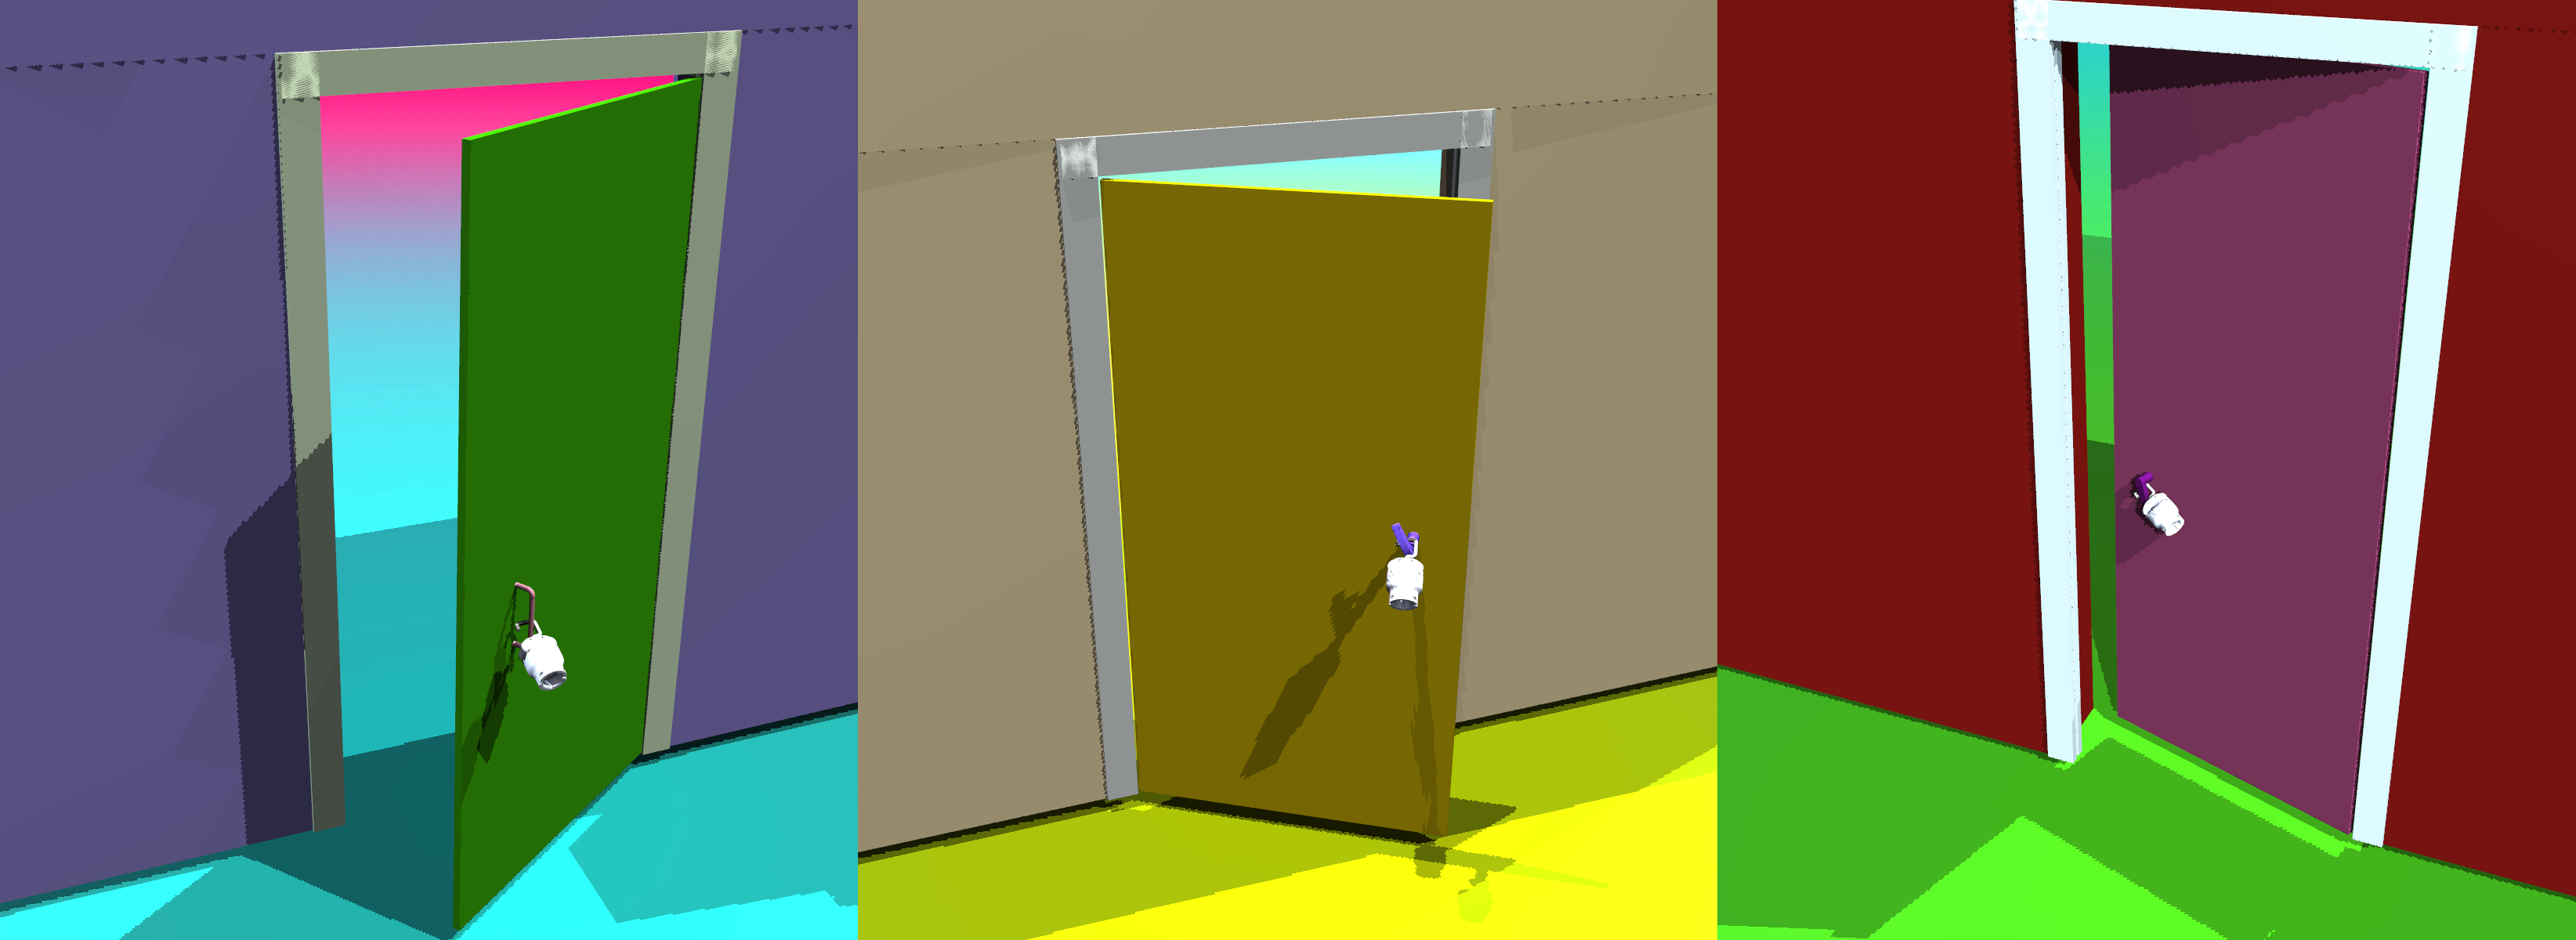
\includegraphics[width=1.0\linewidth]{images/3doors.png}
\end{center}
\caption{Examples of the DoorGym environment and robot. Left: \texttt{pull} handle (task 0); middle: \texttt{lever} handle with left hinge (task 3); right: \texttt{lever} handle with inward (\texttt{push}) opening direction (task 4).}
\label{fig:door-examples}
\end{figure}


\subsection{Metrics}
\label{chap:metrics}
To evaluate the capability of the trained agents, we use the evaluation success rate as the primary metric. In each evaluation, agents are tested on 100 pseudo-randomly picked worlds (of 3000 total), and an opening attempt is deemed successful if the door was opened at least 0.2 rad within 20 seconds of simulation time \citep{doorgym}. Multiple continual learning metrics are derived from the success rates of an agent in different stages of its training.

\paragraph{Continual Learning Metrics} \citet{moreThanForgetting} propose a set of CL metrics based on a train-test accuracy matrix: After training an agent on $N$ tasks, the entries  $\emR_{i,j}$ of the $\mR\in \R^{N\times N}$ accuracy matrix is defined as $\text{accuracy on task }j\text{ after training on task }i$. If $j>i$ and thus the task~$j$ to be evaluated is not known to the hypernetwork, then $i$ is used in the hypernetwork to generate the target network weights (i.e. the embedding of the last known task is used). 
Using the accuracy matrix $A$, forward transfer ($FT$), positive backward transfer ($BWT^+$) and remembering ($REM$) are calculated. The latter 2 are derived from the \textit{backward transfer} $BWT$, but are separated to keep all metrics within $[0,1]$.
\begin{align}
    A =     & \frac{2\sum_{i=0}^n(\sum_{j\leq i}^n\emR_{i,j})}{N(N+1)} \label{eq:accuracy}\\
    FT =    & \frac{2\sum_{i=0}^n(\sum_{j=i+1}^n\emR_{i,j})}{N(N-1)} \label{eq:FT}\\
    BWT =   & \frac{2\sum_{i=1}^n(\sum_{j=0}^{i-1}(\emR_{i,j}-\emR_{j,j}))}{N(N-1)} \label{eq:BTW}\\
    BWT^+ = & max(0, BWT) \label{eq:BWT+}\\
    REM =   & 1-|min(BWT,0)| \label{eq:REM}
\end{align}

\psOLD{Will not report the TFT metric, getting too long. \paragraph{Training Forward Transfer} The CL metrics based on the train-test accuracy matrix only represent the result at the end of an agent's training on a given task. To get insight into the agents' behavior during training time, we also report the forward transfer metric proposed by \citet{continualWorld}. This metric compares the areas under the curve (AUC) for the training curves of the CL method ($\text{AUC}^{cl}$) with a baseline method ($\text{AUC}^{ref}$) for each task $i$. Intuitively, positive forward transfer here indicates faster learning compared to the baseline, while negative forward transfer indicates slowdown and/or a lower final accuracy. To differentiate this metric from the forward transfer derived from the train-test accuracy matrix (Eq. \ref{eq:FT}), we will hereafter refer to it as "training forward transfer" (TFT).
\saOLD{Introduce an abbreviation for this, such as TFT.}
\begin{align}
    TFT = \frac{1}{n}\sum_{i=0}^n \frac{\text{AUC}_i^{cl}-\text{AUC}_i^{ref}}{1-\text{AUC}_i^{ref}} \label{eq:TFT}
\end{align}
}

\section{Experimental evaluation}
\label{chap:experiments}
We conducted multiple experiments to evaluate the ability of \texttt{HN-PPO} to learn the complex dynamics of different door opening tasks. A special focus was set on analyzing how well catastrophic forgetting can be avoided by using a task-conditioned hypernetwork, and whether forward transfer could be observed during the training sequence. All experiments were run three times with different PRNG seeds. Reported values are the mean $\pm$ standard error of the mean of 3 independent results.

\subsection{Baselines}

Table \ref{tab:opening-rates} shows the average after-training opening rates for each task and each method discussed in the following sections. Opening rates are reported at the end of training for a specific task, before any other tasks are visited by the agent. Comparing the results for the non-CL methods (PPO, \mbox{PPO-finetuning}, and \texttt{HN-PPO}+fresh network), the \texttt{pull} doors (task 0 and 1) are the easiest to open, while the \texttt{lever} doors with pull opening direction (task 2 and 3) are the hardest to open.

\begin{table}[tb]
\caption{After-training opening rates per task.}
\label{tab:opening-rates}
\begin{center}
\begin{tabular}{@{}lccccc@{}}
\toprule
Task ID & PPO & PPO-finetuning & \texttt{HN-PPO}+fresh network & \texttt{HN-PPO} & \texttt{HN-PPO+fc} \\ 
\midrule
0 & 1.00 $\pm$ 0.00  & 1.00 $\pm$ 0.00& 0.98 $\pm$ 0.014 & 0.98 $\pm$ 0.014 & 1.00 $\pm$ 0.00\\
1 & 1.00 $\pm$ 0.0027& 1.00 $\pm$ 0.00& 0.97 $\pm$ 0.018 & 1.00 $\pm$ 0.00  & 1.00 $\pm$ 0.00 \\
2 & 0.32 $\pm$ 0.26  & 0.00 $\pm$ 0.00& 0.27 $\pm$ 0.22  & 0.92 $\pm$ 0.014 & 0.69 $\pm$ 0.21\\
3 & 0.32 $\pm$ 0.25  & 0.00 $\pm$ 0.00& 0.25 $\pm$ 0.20  & 0.31 $\pm$ 0.25  & 0.36 $\pm$ 0.23\\
4 & 0.96 $\pm$ 0.014 & 0.37 $\pm$ 0.23& 0.59 $\pm$ 0.24  & 0.59 $\pm$ 0.24  & 0.25 $\pm$ 0.21\\
5 & 0.63 $\pm$ 0.22  & 0.36 $\pm$ 0.24& 0.69 $\pm$ 0.15  & 0.36 $\pm$ 0.15  & 0.01 $\pm$ 0.011\\
\midrule
Average & 0.71 $\pm$ 0.17 & 0.46 $\pm$ 0.14 & 0.63 $\pm$ 0.17 & 0.69 $\pm$ 0.15 & 0.55 $\pm$ 0.15\\
\bottomrule
\end{tabular}
\end{center}
\end{table}


Tables \ref{tab:cl-metrics-baselines} and \ref{tab:cl-metrics-cl} list the CL metrics (cf. Section \ref{chap:metrics}) for all experiments discussed in the following. The tables are split for layout purposes only. 

\begin{table}[tb]
\caption{Continual learning metrics for baseline experiments. The low accuracies and remembering scores indicate catastrophic forgetting. \jhOLD{What do you think about booktabs style like this?}}
\label{tab:cl-metrics-baselines}
\begin{center}
\begin{tabular}{@{}lccc@{}}
\toprule
Metric & PPO & PPO-finetuning & \texttt{HN-PPO}+fresh network \\
\midrule
Accuracy               & 0.24 $\pm$ 0.035 & 0.20 $\pm$ 0.035 & 0.21 $\pm$ 0.023 \\
Forward transfer       & 0.10 $\pm$ 0.0022& 0.10 $\pm$ 0.028 & 0.03 $\pm$ 0.0021 \\
Pos. backward transfer & 0.00 $\pm$ 0.00  & 0.00 $\pm$ 0.00  & 0.00 $\pm$ 0.00 \\
Remembering            & 0.29 $\pm$ 0.078 & 0.47 $\pm$ 0.060 & 0.32 $\pm$ 0.019 \\
\bottomrule
\end{tabular}
\end{center}
\end{table}

\begin{table}[tb]
\caption{Continual learning metrics for \texttt{HN-PPO} and \texttt{HN-PPO+fc}. Remembering is at its maximum possible value, 1.00, for both methods, indicating no forgetting is taking place.}
\label{tab:cl-metrics-cl}
\begin{center}
\begin{tabular}{@{}lcc@{}}
\toprule
Metric & \texttt{HN-PPO} & \texttt{HN-PPO+fc} \\ 
\midrule
Accuracy               &  0.81 $\pm$ 0.041 & 0.73 $\pm$ 0.080\\
Forward transfer       &  0.052 $\pm$ 0.0095 & 0.04 $\pm$ 0.0054\\
Pos. backward transfer &  0.0015 $\pm$ 0.0013 & 0.00 $\pm$ 0.00018\\
Remembering            &  \textbf{1.00} $\pm$ 0.0024 & \textbf{1.00} $\pm$ 0.0044\\
\bottomrule
\end{tabular}
\end{center}
\end{table}


\paragraph{PPO} The single-task PPO implementation in DoorGym, based on code from \citet{pytorchrl}, was used as a baseline for the performance of individual tasks. Hyperparameters for PPO are taken from \cite{doorgym}. For this baseline, a new agent is created for each task, and only trained on that specific task. We observe that the baseline algorithm reliably learns to solve the tasks with \texttt{pull} handles, but yields unstable results for the more challenging \texttt{lever} handles, depending on the seed being used. In the case of tasks 2, 3 and 5, seed dependence was prominent enough so that the agent completely failed to solve the task for one seed, while it could achieve close to 100\% opening rate using a different seed. Figure~\ref{fig:ppo-baseline-graph} shows the door opening rate of the agents at different points in the training progress. The large differences between seeds can clearly be observed, especially in tasks 2 and 3, which use the \texttt{lever} knob. The average after-training opening rate across all 6 tasks is 71\% (\ref{tab:opening-rates}).
\saOLD{This is where a separate PPO agent is trained on each task, right? Make it more explicit.}


\paragraph{PPO-finetuning} This baseline uses ``standard" PPO as before, but instead of creating a new model for each task in the sequence and training it independently, a single agent is fine-tuned on each task in the sequence. The resulting model from training for one task is then used as a pre-trained model for the next task. Since PPO makes no considerations towards continual learning, fine-tuning of policies learned with PPO serves as a lower baseline for the ability of an agent to retain knowledge of previous tasks.
The opening rates plotted in Figure~\ref{fig:ppo-finetuning-graph} show the expected catastrophic forgetting at the task boundary for some tasks (e.g. between task 1 and 2), but also reveal interesting transfer behaviors. Between task 0 and 1 (both \texttt{pull} handles), only little forgetting of knowledge on task 0 occurs, while task 1 has a zero-shot success rate of 61\% thanks to pre-training on task 0. This is likely due to the high similarity of dynamics for these two tasks. On the other hand, the agents' success rate on the \texttt{lever} tasks (2 and 3) was greatly reduced compared to the PPO baseline. Strikingly, even though no success was achieved in solving the \texttt{lever} task during training, one agent was able to open \texttt{lever} doors after being trained on the subsequent \texttt{lever\_push} task (task 4)\asOLD{be consistent with the task fornts. Also I do not know what those numbers refer to in the figure} interval in Figure~\ref{fig:ppo-finetuning-graph}.

These unexpected observations demonstrate the complex relationships between different door opening tasks, which can potentially be exploited by continual learning. 

\begin{figure}[htbp]
\begin{subfigure}{\linewidth}
    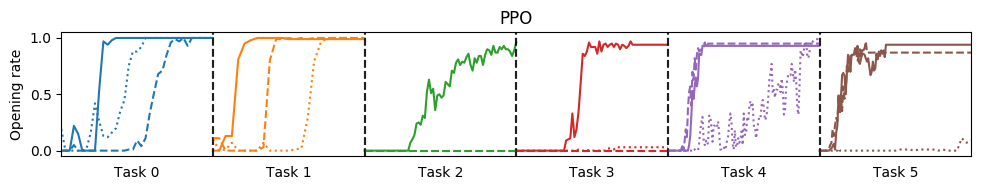
\includegraphics[width=1.0\linewidth]{images/cl_timeseries_series7_config.png}
    \caption{}
    \label{fig:ppo-baseline-graph}
\end{subfigure}
\begin{subfigure}{\linewidth}
    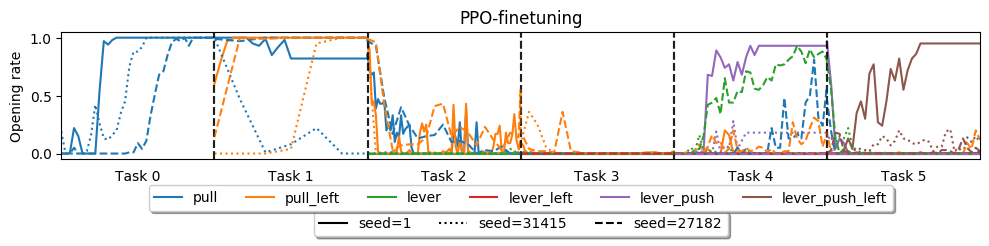
\includegraphics[width=1.0\linewidth]{images/cl_timeseries_series8_config.png}
    \caption{}
    \label{fig:ppo-finetuning-graph}
\end{subfigure}
\caption{Door opening rates using \textbf{(a)} PPO and \textbf{(b)} PPO-finetuning for different door opening tasks and seeds. The x-axis represents the training progress normalized to the longest training run for each task. Progress can thus be compared for multiple training runs of the same task, but not between different tasks. Note that in (a), the sequence of tasks is chosen for consistency with other figures. Each task is trained and evaluated independently.\jhOLD{Instead of plotting all three seeds, how about plotting the median value and a shaded area?}}
\end{figure}

\paragraph{HN-PPO+fresh network} To directly compare the impact of previous experience of a \texttt{HN-PPO} agent on its performance, we train a new \texttt{HN-PPO} agent for each task in this experiment. Like in the PPO baseline, each agent is only trained on a single task, and all agents are trained independently. Since this experiment uses the same network architecture that is used for continual learning, any difference to this baseline is a direct result of an agent's previous experience. Similar to the PPO baseline, large performance differences were again observed between different seeds, as can be seen in Figure~\ref{fig:hnppo_graph_fresh}. The average after-training opening rate is slightly lower than what was achieved by PPO (63\% vs. 71\% for PPO), but within the errors of the respective values (Table~\ref{tab:opening-rates}).


\subsection{Continual Learning Experiments}
\paragraph{HN-PPO}
\label{chap:hnppo}
In this experiment, a single \texttt{HN-PPO} agent was trained sequentially on the tasks in the CL sequence. Figure~\ref{fig:hnppo_graph} shows the opening rate for each of the 6 tasks in the CL sequence during the agents' training. The lack of sharp drops in the opening rate graph clearly indicates that the hypernetwork is able to learn multiple tasks with different dynamics without any significant loss of accuracy in previously seen tasks.  \texttt{HN-PPO} shows excellent protection against catastrophic forgetting, achieving a remembering score of 1.00, as can be seen in Table~\ref{tab:cl-metrics-cl}. This indicates that on average, no skill was lost by learning additional skills. The method also achieves very similar after-training opening rates to the PPO baseline (Table~\ref{tab:opening-rates}), which confirms that the CL capabilities do not adversely affect PPO's single-task performance. While there is virtually no forgetting, significant backward transfer does also not occur. This result is expected, since the hypernetwork regularization aims to minimize changes to previously learned dynamics, both beneficial and detrimental.

\begin{figure}[tb]
\begin{subfigure}{\linewidth}
    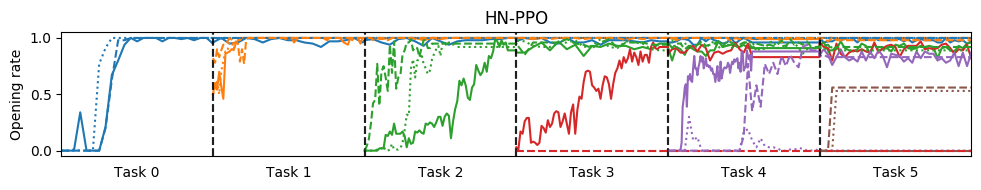
\includegraphics[width=1.0\linewidth]{images/cl_timeseries_series5_config.png}
    \caption{}
    \label{fig:hnppo_graph}
\end{subfigure}
\begin{subfigure}{\linewidth}
    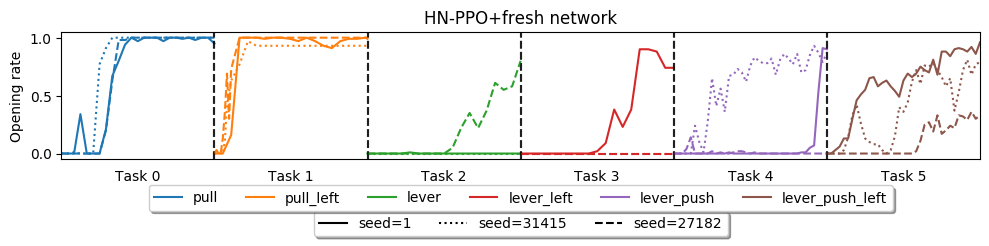
\includegraphics[width=1.0\linewidth]{images/cl_timeseries_series6_config.png}
    \caption{}
    \label{fig:hnppo_graph_fresh}
\end{subfigure}
\caption{\textbf{(a)} Door opening rates using \texttt{HN-PPO}, \textbf{(b)} \texttt{HN-PPO} with a fresh network for each task.\jhOLD{the data for this plot (a) are still incomplete, right?}}
\end{figure}

\paragraph{Fresh Critic}
\label{chap:freshcritic}
In this experiment, a modified \texttt{HN-PPO} agent is used, which only parameterizes the actor network with a hypernetwork. The critic network on the other hand is freshly initialized for each task. This alternative architecture, \texttt{HN-PPO+fc}, is then trained on the CL task sequence in the same way as the \texttt{HN-PPO} agent. Compared to standard \texttt{HN-PPO}, the after-training opening rate is 20\% lower (55\%, vs. 69\% for \texttt{HN-PPO}) and the CL accuracy is 10\% lower (73\%, vs. 81\% for \texttt{HN-PPO}). Importantly though, we find that \texttt{HN-PPO+fc} exhibits the same, highly effective protection against catastrophic forgetting as \texttt{HN-PPO}, also having a remembering score of 1.00. 
 
\begin{figure}[tb]
\begin{center}
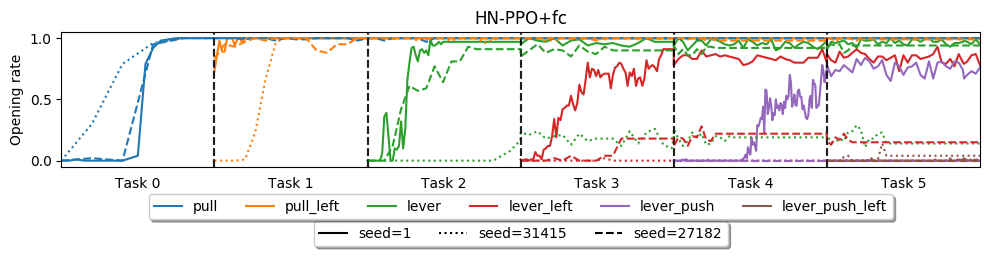
\includegraphics[width=1.0\linewidth]{images/cl_timeseries_series4_config.png}
\end{center}
\caption{Door opening rates using HN-PPO+fc.
\saOLD{Isn't this result only for 1 seed? I think we should show the results for the other seeds as well.} \psOLD{obviously, more data is coming ;)}
}
\label{fig:hnppo+fc-graph}
\end{figure}

\subsection{Regularizer Ablation Study}
\label{chap:ablation}
In this experiment, we aim to investigate the importance of regularizing the weights of previously learned tasks. Experiments were run with the same hyperparameters and environments as in Section \ref{chap:hnppo}, but regularization of the hypernetwork outputs on previous task embeddings was disabled by setting $\beta=0$ (cf. Eq. \ref{regloss}). Removing hypernetwork regularization resulted in a 67\% decrease in average accuracy, as well as a 76\% decrease in remembering of previous tasks, as can be seen in Table~\ref{tab:ablation-results}. 

\begin{table}[tb]
\caption{Effects of hypernetwork regularization on continual learning}
\label{tab:ablation-results}
\begin{center}
\begin{tabular}{@{}lcc@{}}
\toprule
Algorithm & \texttt{HN-PPO+fc} & \texttt{HN-PPO+fc}, no regularization \\ 
\midrule
Accuracy               &  \textbf{0.73} $\pm$ 0.080 & 0.24 $\pm$ 0.038\\
Forward transfer       &  0.04 $\pm$ 0.0054 & 0.03 $\pm$ 0.012\\
Pos. backward transfer &  0.00 $\pm$ 0.00018& 0.00 $\pm$ 0.00\\
Remembering            &  \textbf{1.00} $\pm$ 0.0044& 0.24 $\pm$ 0.076\\
\bottomrule
\end{tabular}
\end{center}
\end{table}

Without regularization, the near-perfect remembering of previous tasks seen in \texttt{HN-PPO+fc} drops even below the PPO-finetuning baseline (cf. Table~\ref{tab:cl-metrics-baselines}). This result confirms that while hypernetworks provide the model with the necessary capacity and flexibility, regularization of the hypernetwork outputs is mainly responsible for their high resilience against catastrophic forgetting.

\section{Discussion}
\asOLD{Start with summarizing what you did, this paragraph comes as too abrupt.} 
In our experiments, we have shown that our \texttt{HN-PPO} agent can successfully learn to open up to 6 different types of doors. While \citet{MBRLHypernetworks} have demonstrated that hypernetwork-based CL is able to consistently achieve high returns on multiple DoorGym tasks, our work shows that this capability also extends to fully solving the task at hand, i.e. opening the door. To this end, we chose to use the door opening success rate (cf. Section~\ref{chap:metrics}) as the main performance indicator, in contrast to \citet{MBRLHypernetworks}, who report the average return as the core metric. We argue that in a scenario with a clear final goal, such as door opening, the success rate better represents the quality of a policy. The training time until a door can be reliably opened is however significantly longer than what \citet{MBRLHypernetworks} experimented with. In their experiments, agents were trained for 60.000 environment steps per task, while we trained for up to $2.4*10^7$ environment steps per task. 

%\asOLD{Part of this paragraph, specially the last sentences would go better in the discussion}. 
The distinction between these 2 metrics is further motivated by our discovery that under certain circumstances, the evaluation return of the DoorGym environment is not representative of the ability of an agent to solve the task. Similar returns in the same environment can correspond to vastly different opening rates, as shown in Figure~\ref{fig:return_opening_rate}. While the three return curves follow a similar pattern, one agent is able to solve the task with a high opening rate, while the other 2 are unsuccessful.

\begin{figure}[htbp]
\begin{center}
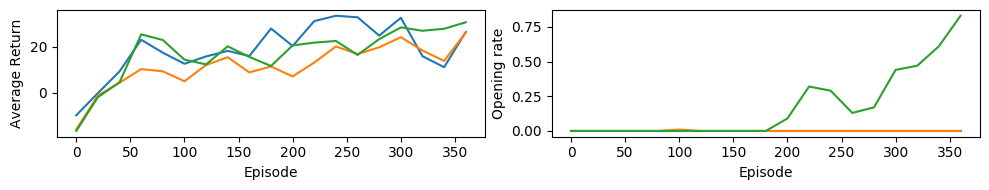
\includegraphics[width=1.0\linewidth]{images/return_opening_rate.png}
\end{center}
\caption{Return-opening rate mismatch: Evaluation return and opening rate curves of 3 experiments in the same environment (\texttt{HN-PPO}+fresh network, \texttt{lever} task).}
\label{fig:return_opening_rate}
\end{figure}

Interestingly, the choice of the time point to end an agent's training on one task does sometimes greatly affect downstream tasks. Even when convergence is reached for key metrics (opening rate, average return), an agent might not be able to learn a following task when starting from one checkpoint, but succeed in doing so when starting from an earlier or later checkpoint. This hidden ability of a hypernetwork to learn further tasks may be of interest for further research. Avoiding states in which the learning of future tasks is hindered will help to further improve the capabilities of hypernetworks in CL.
%\saOLD{Elaborate a bit more. The message is not completely clear here.}
%\saOLD{Add plots for the returns as well, and discuss the finding about returns being good for all seeds but not the success rate. If possible, include an image or a link to a video showing the opening of doors.}
%\jhOLD{sounds very interesting}
\section{Conclusions, Limitations and Outlook}
\label{chap:conclusion}
%\jhOLD{\url{https://towardsdatascience.com/how-you-should-read-research-papers-according-to-andrew-ng-stanford-deep-learning-lectures-98ecbd3ccfb3} Andrew Ng suggests to read research papers in multiple passes; search for %"first pass" in the blog post: "In your first pass, start with reading the following sections within the paper: title, abstract and figures."
%"The second pass entails you reading the following sections: introduction, conclusion, another pass through figures and scan through the rest of the content."}
%\jhOLD{So the introduction, conclusion, abstract and figure captions should be read without the text and provide insight. 
%So I think you need describe a bit more what we're doing in the conclusion; for example, mention again what is learned in a continual way; (i.e. a policy that can then solve multiple tasks, and the continual learning is in %the tasks);}
We presented \texttt{HN-PPO}, a novel approach to continual RL using PPO and a hypernetwork-based policy network. Using our method, the agent learns a policy for solving multiple tasks via a task-conditioned hypernetwork. New tasks can be trained in a continuous setting. The hypernetwork size is almost constant: it only grows by the size of the task embedding vector, which is only 8-dimensional in our experiments. This enables our method to scale to high numbers of tasks. In our experiments, we demonstrated that \texttt{HN-PPO} is a highly effective method to learn multiple tasks with complex dynamics, while offering strong protection against catastrophic forgetting. We compared two network architectures; a shared-parameters actor-critic using a hypernetwork, and an architecture with a non-hypernetwork critic. While we found the shared-parameter architecture to achieve slightly higher average accuracy, both methods protect well against catastrophic forgetting. Further, our experiments show that regularization of the task-conditioned hypernetwork outputs is crucial for avoiding catastrophic forgetting. 

While highly capable, \texttt{HN-PPO} suffers from training instability. This instability is also present in the PPO baseline, but is amplified by training the same agent on multiple tasks, which results in very long total training times. When using default PPO hyperparameters for \texttt{HN-PPO}, gradient explosions randomly occurred in some experiments. Training was stabilized to an acceptable level after reducing the maximal gradient norm from 0.5 to 0.0001 (cf. Table~\ref{tab:hnppo-hparams}). The choice of random seed also greatly influences the training outcome, which is another indicator of said instability. Additionally, the choice of training stop point is also of importance for good performance downstream, however, it remains unclear how to find the optimal stopping point under this aspect. Considering these limitations, reducing training instability should be an objective of further research on this subject. Understanding the causes for the variability in downstream performance could also significantly aid our line of work. Finally, the current method requires long training times of up to 1~day per task, which makes experiments with very long task sequences unpractical. Attempting to optimize \texttt{HN-PPO}'s convergence behavior and computational efficiency may therefore be of interest as well.
%\saOLD{Talking about the limitations is an important part of the paper. Please elaborate a bit more.}


\bibliography{iclr2023_conference}
\bibliographystyle{iclr2023_conference}

\appendix
\section{Appendix}
\subsection{Experiment Details}
\paragraph{HN-PPO Hyperparameters}
Table~\ref{tab:hnppo-hparams} lists the hyperparameters used for experiments with \texttt{HN-PPO} and \texttt{HN-PPO+fc}. $\beta$ and the task embedding dimension are specific to HN-PPO, the other were adapted from DoorGym's default values for PPO \citep{doorgym}. 

\begin{table}[htbp]
\caption{\texttt{HN-PPO} hyperparameters}
\label{tab:hnppo-hparams}
\begin{center}
\begin{tabular}{@{}ll@{}}
\toprule
Name & Value \\ 
\midrule
Hypernetwork regularization $\beta$ (Eq. \ref{regloss})& 0.001 \\
Task embedding dimension & 8 \\
Learning rate & 0.005 \\
Parallel rollouts & 8 \\
PPO mini-batch size & 256 \\
PPO clipping parameter $\epsilon$ (Eq. \ref{ppo-clip}) & 0.3 \\
Max. gradient norm & 0.0001 \\
Reward discount ratio $\gamma$ & 0.99\\
GAE lambda & 0.95\\
Entropy bonus coeff. $c_e$ (Eq. \ref{ppo-actorcritic}) & 0.01\\
Value loss coeff. $c_v$ (Eq. \ref{ppo-actorcritic}) &  0.5\\
\bottomrule
\end{tabular}
\end{center}
\end{table}


\paragraph{Network Architecture}
\label{chap:architecture}
For PPO, the default DoorGym network architecture was reused: Both actor and critic networks are modeled as MLPs with 2 hidden layers of 64 neurons each. $tanh$~was used as the activation function. The critic network has an output dimension of 1 (the scalar value of the action), the actor has an output dimension of 6 (each controlling an input to the 6-DoF \texttt{floatinghook} robot). During training, a stochastic policy is used, with actions sampled from a normal distribution parameterized by the actor's output (mean) and a learned standard deviation vector. In evaluation, actions are taken directly from the actor's output, making the policy deterministic.

In \texttt{HN-PPO}, the target networks have the same architecture as laid out above for PPO. The hypernetwork controlling their weights is an MLP with 2 hidden layers of 640 \saOLD{or 64?} \psOLD{640 is correct, it's 10x the TN size} neurons each. In the hypernetwork, ReLU activation is used for the hidden layers. The output layer of the hypernetwork is a multi-head (blue in Figure~\ref{hnet-arch}) with no non-linearity applied. Each head represents one tensor containing parameters of the target network, with output dimensions chosen accordingly. For the actor shown in Figure~\ref{hnet-arch}, 7 heads are generated: a weight and bias tensor for each layer, plus an additional standard deviation vector for the Gaussian stochasticity layer. Accordingly, the shown critic network requires 6 heads to parameterize.\\
For the "fresh critic" (\texttt{HN-PPO+fc}) architecture (cf. Section~\ref{chap:freshcritic}), the critic is not parameterized by the hypernetwork, but is a stand-alone MLP. Accordingly, the number of output heads in the hypernetwork is reduced.

\saOLD{I think this can be moved into the methods section.} \psOLD{Is here because it's one of the first things to go if I exceed the length. Will move depending on space requirements at the end}

\begin{figure}[htbp]
\begin{center}
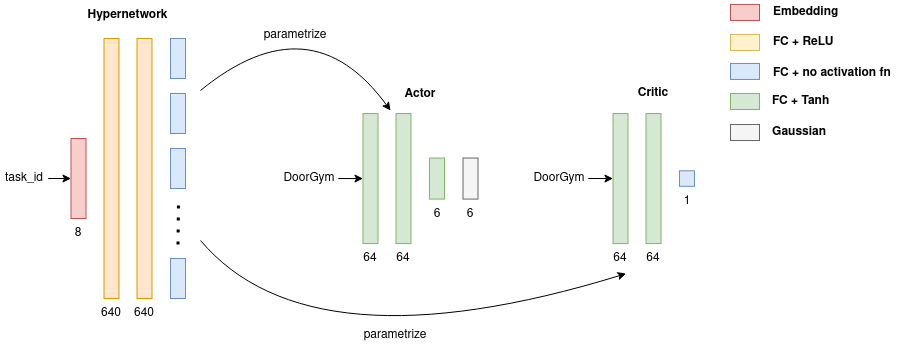
\includegraphics[width=0.8\linewidth]{images/hnet_arch.png}
\end{center}
\caption{Network architecture in HN-PPO.}
\label{hnet-arch}
\end{figure}

\subsection{Supplementary Information}
\paragraph{Accuracy Matrices}
In this section, we show the train-test accuracy matrices, from which the CL metrics in Section~\ref{chap:metrics} are calculated \citep{moreThanForgetting}. For each training setup, we show the element-wise average matrix of 3 experiments. Matrix entry $\emA_{i,j}$ represents the opening rate for an agent at the end of its training for task $i$, evaluated on task $j$. 

\begin{itemize}
\item PPO:
\[\left[\begin{array}{cccccc}
1.0& 0.21& 0.0& 0.0& 0.0& 0.0\\
0.48& 1.0& 0.0& 0.0& 0.0& 0.03\\
0.11& 0.01& 0.32& 0.0& 0.57& 0.0\\
0.0& 0.29& 0.0& 0.32& 0.0& 0.62\\
0.0& 0.01& 0.0& 0.0& 0.96& 0.0\\
0.01& 0.01& 0.0& 0.0& 0.0& 0.63
\end{array}\right]\]

\item PPO-finetuning:
\[\left[\begin{array}{cccccc}
1.0& 0.21& 0.0& 0.0& 0.0& 0.0\\
0.61& 1.0& 0.0& 0.0& 0.0& 0.0\\
0.0& 0.24& 0.0& 0.0& 0.53& 0.0\\
0.0& 0.01& 0.0& 0.0& 0.0& 0.68\\
0.19& 0.06& 0.27& 0.0& 0.37& 0.0\\
0.01& 0.05& 0.0& 0.0& 0.0& 0.36
\end{array}\right]\]

\item \texttt{HN-PPO}+fresh network
\[\left[\begin{array}{cccccc}
0.98 & 0.39 & 0.0 & 0.0 & 0.0 & 0.0 \\
0.18 & 0.97 & 0.0 & 0.0 & 0.01 & 0.0 \\
0.23 & 0.0 & 0.27 & 0.0 & 0.0 & 0.0 \\
0.0 & 0.02 & 0.0 & 0.25 & 0.0 & 0.0 \\
0.0 & 0.0 & 0.02 & 0.0 & 0.59 & 0.0 \\
0.0 & 0.08 & 0.0 & 0.03 & 0.0 & 0.69\\
\end{array}\right]\]

\item \texttt{HN-PPO}
\[\left[\begin{array}{cccccc}
0.98 & 0.39 & 0.0  & 0.0  & 0.0  & 0.0\\
0.99 & 1.0  & 0.0  & 0.0  & 0.0  & 0.0\\
1.0  & 1.0  & 0.92 & 0.01 & 0.0  & 0.0\\
0.99 & 1.0  & 0.93 & 0.31 & 0.0  & 0.39\\
0.99 & 1.0  & 0.92 & 0.28 & 0.59 & 0.0\\
0.99 & 0.99 & 0.92 & 0.27 & 0.57 & 0.36\\
\end{array}\right]\]

\item \texttt{HN-PPO+fc}:
\[\left[\begin{array}{cccccc}
1.0& 0.45& 0.0& 0.0& 0.01& 0.0\\
1.0& 1.0& 0.0& 0.0& 0.0& 0.0\\
1.0& 1.0& 0.69& 0.0& 0.0& 0.0\\
1.0& 1.0& 0.69& 0.36& 0.0& 0.16\\
1.0& 0.99& 0.7& 0.34& 0.25& 0.0\\
1.0& 1.0& 0.68& 0.31& 0.25& 0.01
\end{array}\right]\]

\item \texttt{HN-PPO+fc}, no regularization:
\[\left[\begin{array}{cccccc}
1.0& 0.45& 0.0& 0.0& 0.01& 0.0\\
0.66& 1.0& 0.0& 0.0& 0.0& 0.01\\
0.33& 0.0& 0.44& 0.0& 0.0& 0.0\\
0.0& 0.03& 0.0& 0.62& 0.0& 0.0\\
0.0& 0.0& 0.0& 0.0& 0.83& 0.0\\
0.0& 0.01& 0.0& 0.0& 0.0& 0.04
\end{array}\right]\]
\end{itemize}

\paragraph{Code availability} The code used to run the experiments is available under \url{https://git.uibk.ac.at/csas8782/schoepf-bachelor-thesis}.
\end{document}


\begin{table}[tb]
\caption{CW metrics table. TODO: Should not be included in final version.}
\label{tab:cw-results}
\begin{center}
\begin{tabular}{@{}lc@{}}
\toprule
Metric & Value \\ 
\midrule
Avg. performance           &  0.68 $\pm$ 0.049\\
Training forward transfer  &  0.33 $\pm$ 0.040\\
Forgetting                 &  0.0089 $\pm$ 0.0039\\
\bottomrule
\end{tabular}
\end{center}
\end{table}